% Generated from paper/source. Do not edit by hand.
\section{Ablations}
\subsection{Noncommutative order}
The commutative complex accumulator retains a complex state and magnitude-squared readout but sums evidence injections. Its in-domain top-1 is 0.704, moderate-shift top-1 is 0.415, and chronology-pair accuracy is zero. The full complex operator reaches 0.969, 0.647, and 1.000. The paired shift effect is +0.232 with its three-world interval above zero. This is the largest critical ablation and confirms that ordered operator composition, not complex storage alone, is necessary for the leading result.

The control is intentionally algebraic. Because addition commutes, it cannot encode the marker order. A performance collapse on pairs is therefore expected, while the moderate-shift loss shows that chronology-related sequential structure also contributes to the broader shifted set. It remains possible that a different ordered real architecture could reproduce the result; the ablation establishes necessity within Q-Neuro, not exclusivity across all computation.

\subsection{Phase-sensitive measurement}
The two-channel real control reaches 0.499 moderate-shift top-1 and 0.663 pair accuracy. The complex operator adds +0.148 shift accuracy. The phase-insensitive magnitude readout retains the full complex recurrence but forbids destructive readout interference; it reaches 0.543 shift top-1 and 0.825 pairs, leaving a +0.104 gap to the full model. Phase-sensitive measurement is therefore functionally important under the trained law.

This result is stronger than post hoc phase scrambling because the ablated model is retrained. It is still not a theorem about complex arithmetic. A sufficiently general real network can represent complex multiplication using paired channels. The finding is that the tested complex parameterization provides a useful bias relative to the declared controls at this scale.

\subsection{Observed-negative evidence}
Removing the negative-evidence channel reduces shift top-1 from 0.647 to 0.575 and chronology-pair accuracy from 1.000 to 0.972. The +0.072 shift effect has an interval above zero. The ablation also worsens ambiguity NLL to 3.274. Negative findings therefore provide more than missingness; they shape both elimination and uncertainty.

Observed-negative tokens are not yet diagnosis-conditional contradiction operators. They are learned tokens whose effects emerge through supervised training. A stronger causal study would intervene on matched positive/negative evidence for each latent factor and test monotonicity at the state and probability levels.

\begin{figure}[t]
\centering
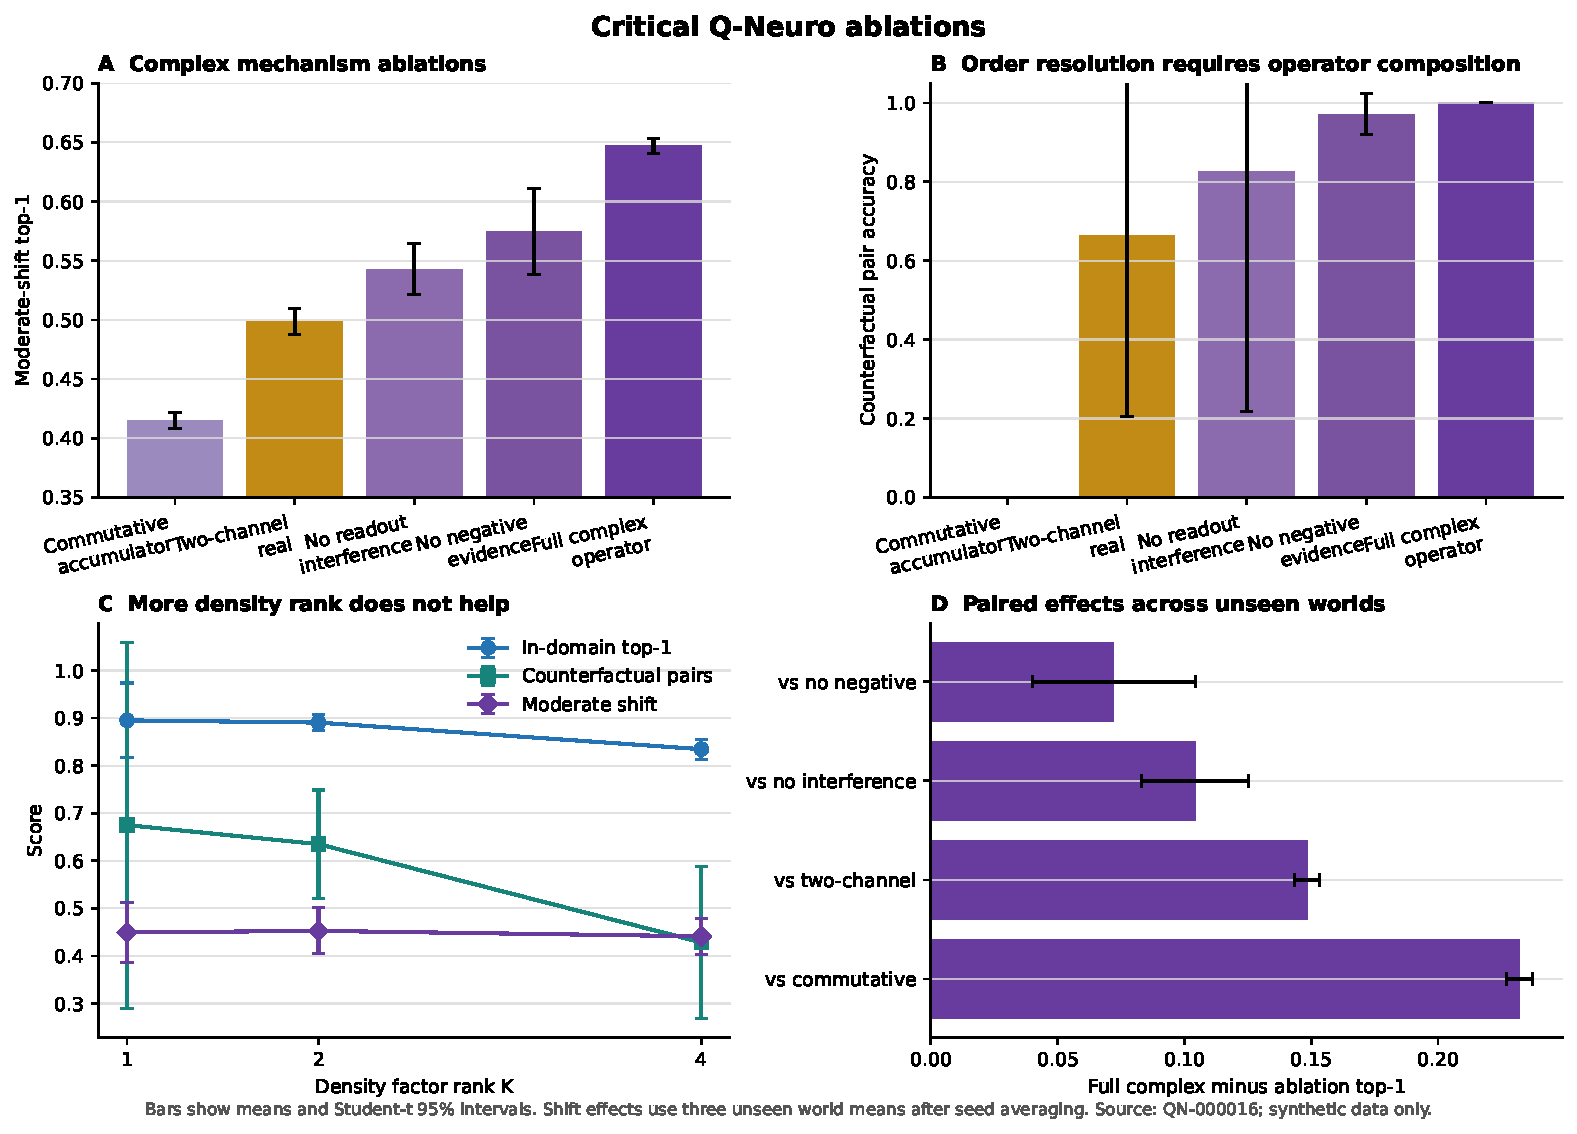
\includegraphics[width=0.98\linewidth]{figures/critical_ablation_suite.pdf}
\caption{Removing ordered composition produces the largest robustness and chronology loss. Phase-insensitive measurement and removal of observed-negative evidence also degrade the full complex model. Density rank does not improve the tested frontier.}
\label{fig:critical_ablation_suite}
\end{figure}

\input{tables/critical_ablations.tex}

\subsection{Coherence and dissipation}
The Hamiltonian-style model reaches 0.556 moderate-shift top-1 and 0.983 chronology-pair accuracy. Dissipative-only evolution reaches 0.438 and 0.008. Their hybrid reaches 0.550 and 0.923. Hybrid-minus-dissipative is +0.112 with a narrow three-world interval, while hybrid-minus-Hamiltonian is --0.006 with an interval crossing zero. Generic learned damping is not an automatic model of diagnostic elimination.

The most plausible explanation is architectural: elementwise damping plus normalization can erase path information without targeting a contradicted hypothesis. The result does not reject all dissipative or Lindblad-like laws. It rejects this generic parameterization under this objective and suggests that future dissipation must be diagnosis-conditional and compared against a matched removal operator.

\subsection{Density rank}
Density ranks one, two, and four reach 0.449, 0.453, and 0.441 moderate-shift top-1. Rank four uses more parameters but lowers source accuracy, worsens ambiguity NLL, and reduces chronology-pair accuracy. Off-diagonal capacity is therefore not automatically useful when supervision sees only the diagonal diagnosis measurement.

The invariant checks still matter: every tested density state is Hermitian, positive semidefinite, and unit trace within numerical tolerance. What fails is the predictive hypothesis. A later-resolution task or multi-observable objective could make off-diagonal structure identifiable; the present benchmark does not.

\subsection{Ambiguity differential}
The real operator’s advantage on ambiguity is not a small calibration detail. It assigns nearly four times as much mass to the valid twin set as the complex model and is much closer to the theoretical pair NLL floor. Meanwhile, the complex model leads source and shifted top-1. The result exposes a central design tension between sharp order discrimination and calibrated coexistence of unresolved hypotheses.

\begin{figure}[t]
\centering
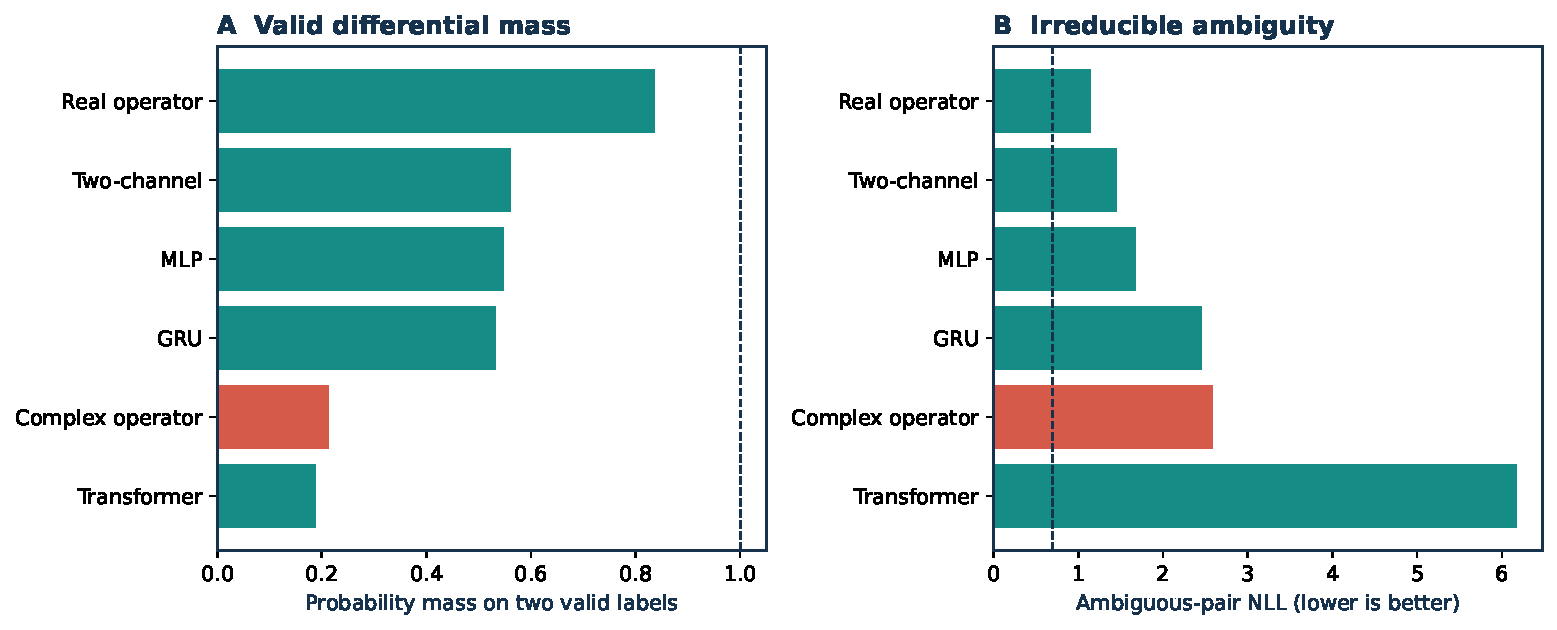
\includegraphics[width=0.98\linewidth]{figures/ambiguity_differential.pdf}
\caption{The real operator retains substantially more probability mass on the two valid ambiguity labels, while the complex operator has worse pair NLL despite stronger shifted classification accuracy.}
\label{fig:ambiguity_differential}
\end{figure}

An ambiguity-aware loss could directly supervise a valid label set or impose a distribution over equivalence classes. Such a loss would change the problem and must be evaluated for accuracy tradeoffs. The architecture alone does not guarantee metastable differentials.

\subsection{Ablation interpretation}
The ablations support a constrained mechanism chain: signed evidence enters in order; noncommuting composition preserves chronology; complex phase participates in the readout; and the resulting parameterization is robust to the declared shifts. They do not support a physical quantum interpretation, a unique representation theorem, or a claim that coherence is inherently beneficial. The density and dissipation failures are especially important because they show that adding more quantum-inspired structure can make the system worse.
